\documentclass[12pt, a4paper]{report}
\usepackage[utf8]{inputenc}
%subpackage
\usepackage{subcaption}
\usepackage{float}
% hyperref
\usepackage[bookmarks, colorlinks, breaklinks]{hyperref}  % PDF hyperlinks, with coloured links
\hypersetup{linkcolor=black, citecolor=black, filecolor=black, urlcolor=black} % black links, for printed output

% Support for the inclusion of figures
\usepackage{graphicx}

% "Contents" and "bibliography" are included in the summary.
\usepackage{tocbibind}

% Packages and configuration for Alloy code listing
%\usepackage{listings}
%\usepackage{alloy}
%\usepackage{color}
%\definecolor{alloy-keyword}{rgb}{0.23, 0.23, 0.7}
%\definecolor{alloy-comment}{rgb}{0.18, 0.64, 0.18}
%\definecolor{alloy-string}{rgb}{0.71, 0.18, 0.71}

\def\chapterautorefname{Chapter}

\begin{document}
\title{Software Engineering 2: TrackMe \\ \vspace{1em} Design Document}
\author{Haritha Harikumar, Mohini Gupta, Saloni Kyal\\
Politecnico di Milano}
\date{December 10, 2018}
\maketitle
\tableofcontents

%%%%%% INTRODUCTION %%%%%%%%
\chapter{Introduction}
\label{ch:introduction}

\section{Purpose}
TrackMe is an android application developed by TrackMe. The application helps to monitor health vitals and location of individuals. TrackMe stands apart from other health monitoring application with its features that enables 3rd party services to monitor the data of individuals for a valid cause. TrackMe also provides other useful services like emergency alerts to ambulances in case an individual's vitals are in critical condition. Apart from that TrackMe comes with a service which offers people or a group of people to organise and visualise races or marathons. 

This document is intended to be examined by a group of developers that will implement our system to make the implementation consistent with the system project.



\section{Scope}
\qquad Track4Me is a company which provides three software based services. The services are limited to the citizens of Milan. The given problem is to design and develop a software service called  “Data4Help”,  which acts as an intermediary between the individuals and the other companies. It targets two set of users, individuals and third party. The location and health of the user is extracted from a wearable device. The data from the wearable device is extracted with the help of the API of the wearable device. The software tracks the location and health status of individuals or group of individuals and send the information to the third party on their request to monitor the health of individuals by validating the type of requests. The validation of the requests for the information of specific individuals is done by the individual’s self acceptance or rejection. The requests for the information of group of individuals is decided by Track4Me and generalized by allowing the access to the third party, if the number of individuals whose information is to be accessed is greater than 1000.

\qquad It builds a new service called “AutomatedSOS” over the top of “Data4Help” after monitoring the demand of requests from third parties for giving non-intrusive SOS service to elderly people, which sends the ambulance to individual’s location when the health parameters are below the thresholds. The nearest ambulance is tracked and sent to ensure individual’s quick and efficient recovery. A separate mobile application of Track4Me is to be exclusively developed for the ambulance drivers who are informed by push notifications in the mobile application along with the location and other details of the patient in less than 5 seconds to ensure spontaneity in reaction to emergencies. All the hospitals in Milan are informed to ensure all the ambulance drivers installs TrackMe application.

\qquad A new service called “Track4Run” is built as a source of revenue which allows organizer to organize an event, athletes to participate in the event and spectators to see the athletes position live in a Map. It exploits the service of “Data4Help” which tracks the location of the athletes to be visible to everyone and helps the organizer to monitor the health status of athletes as well. The organize will be registered as an existing or new third-party. The athletes will be registered as existing or new individual and the spectators can be registered as new/existing individual/third party.

\qquad The users can either register as an individual or as an organization/company(third party).Data4Help is a base service which all the individuals and third party will have by default even if the user registers for a different service other than “Data4Help”. The third party can register for two services: “Data4Help” and “Track4Run”. It uses “Data4Help for receiving information about targeted individuals and “Track4Run to organize events for a particular cause/occasion. The third party is a source of revenue for both cases, as Track4Me provides information about individuals and thereby,  provides customers to their organization which brings them profit. Individuals can register for any of the three services. The first service is a free service  with a motive to help them to receive specific input from respective third party for their health issues or other factors. The individual can also upgrade to other services if they are an existing a member using one service by making payment. Payment can be made using PayPal or a credit card. Track4Me guarantees the security of the individuals data and only associates with trusted third party companies. Ultimately, it helps both individuals and third party to manage and monitor their personal data and aims at being a robust and efficient software


\section{Definitions, Acronyms, and Abbreviations}
\subsection{Definitions}
\begin{enumerate}
\end{enumerate}

\subsection{Acronyms}
\begin{enumerate}
\item DD: Design Document
\item API: Application Program Interface
\item DBMS: Data Base Management System
\item SOS: Save our Souls
\item GPS: Global Positioning System
\item GUI: Graphical User Interface
\item RASD: Requirement Analysis and Specification Document
\end{enumerate}

\subsection{Abbreviations}
\begin{enumerate}
\item Gn: n-Goals
\item An: n-Assumptions
\item Dn: n-Dependencies
\item Cn: n-Constraints
\item Rn: n-Functional Requirement s
\end{enumerate}


\section{Document Structure}
\qquad The DD is composed of 6 parts including references
\begin{enumerate}
\item Chapter 1: Introduction
\item Chapter 2: Architectural Design
\item Chapter 3: User Interface Design
\item Chapter 4: Requirements Traceability
\item Chapter 5: Implementation, Integration and test plan
\item Chapter 6: Effort Spent
\end{enumerate}

%%%%%% Architectural Design %%%%%%%%
\chapter{Architectural Design}
\label{ch:architectural_design}

\section{Overview}
\qquad The TrackMe application has the following architecture. 

\section{Component View}
In the following diagram, the mentioned components are more closely examined, with the main focus on the application server. While describing the parts, the notation will be the interface they are providing in order to be more general, because there may be one or more different implementations of the same service within the server. The components shown here communicate with each other and work together to complete certain user requests.\newline\newline
\textbf{DATA4HELP SERVICE}
\begin{figure}[H]
	\begin{center}
		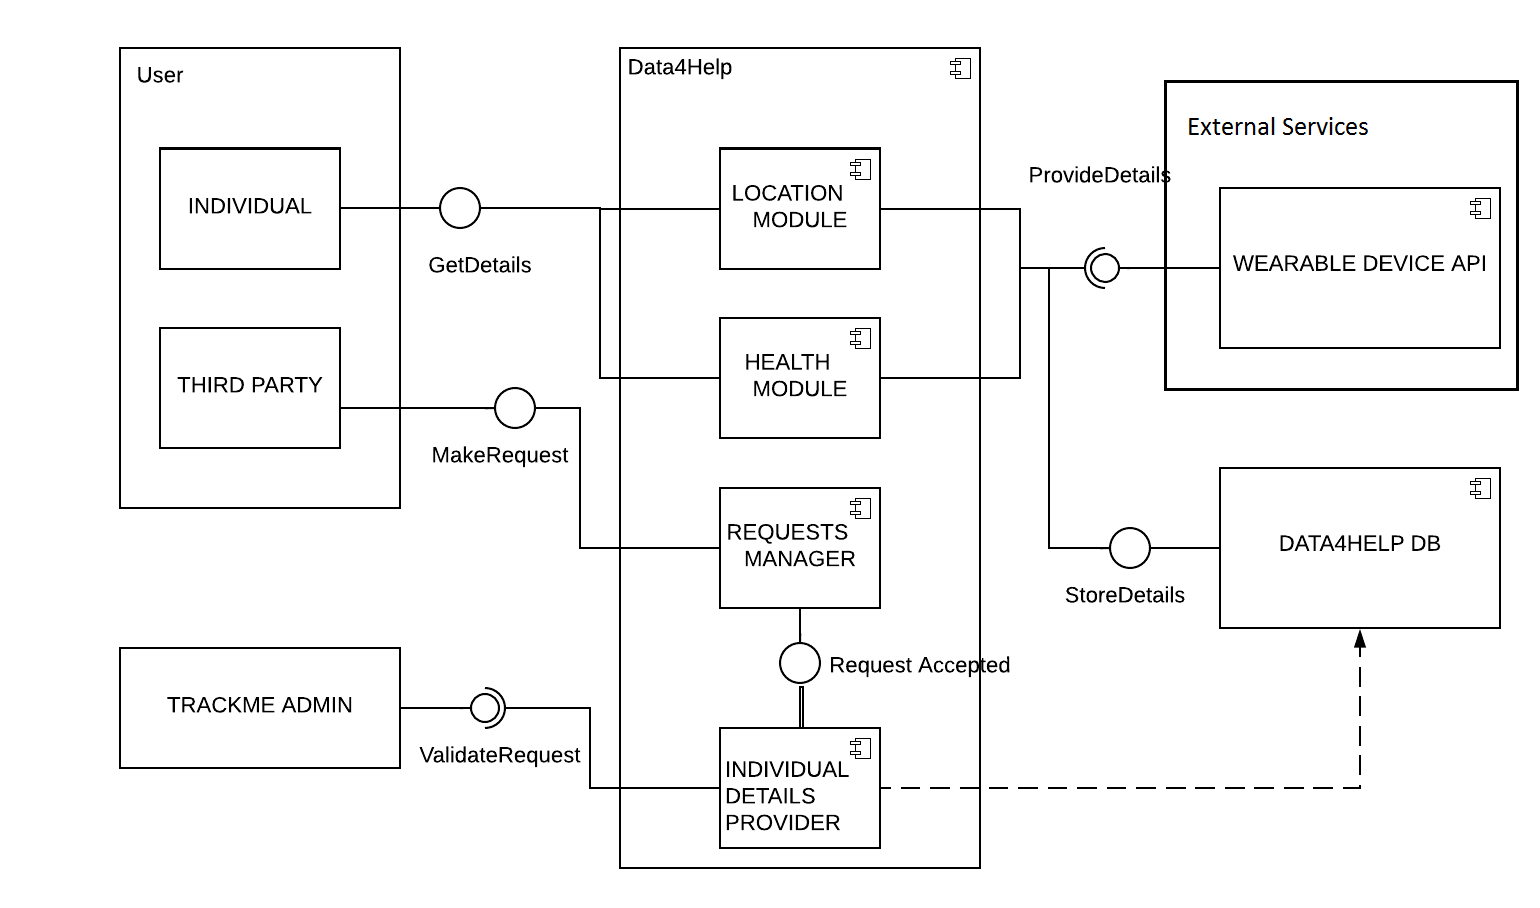
\includegraphics[width=\textwidth]{./DD_Diagrams/ComponentData4Help.png}
      	\caption{Component Diagram for Data4Help Service}
        \label{TrackMe_c1}
	\end{center}
\end{figure}

\begin{itemize}
\item\textbf{Location module:}  the location fetched from the Wearable Device API provided by an Individual is stored in the Data4Help DB.
\item\textbf{Health module:}  the health values fetched from the Wearable Device API provided by an Individual is stored in the Data4Help DB.
\item\textbf{Request Manager:}  provides an interface to the Third Party to make new request to get the details of a specific Individual or a group of Individual. It also provides an interface to a specific Individual to accept or reject the request.
\item\textbf{Individual Details Provider:} this uses the  help of the Data4Help DB to provide the details to the Third Party after the TrackMe Admin has validated the request.
\newline
\end{itemize}
\textbf{AUTOMATEDSOS SERVICE}
\begin{figure}[H]
	\begin{center}
		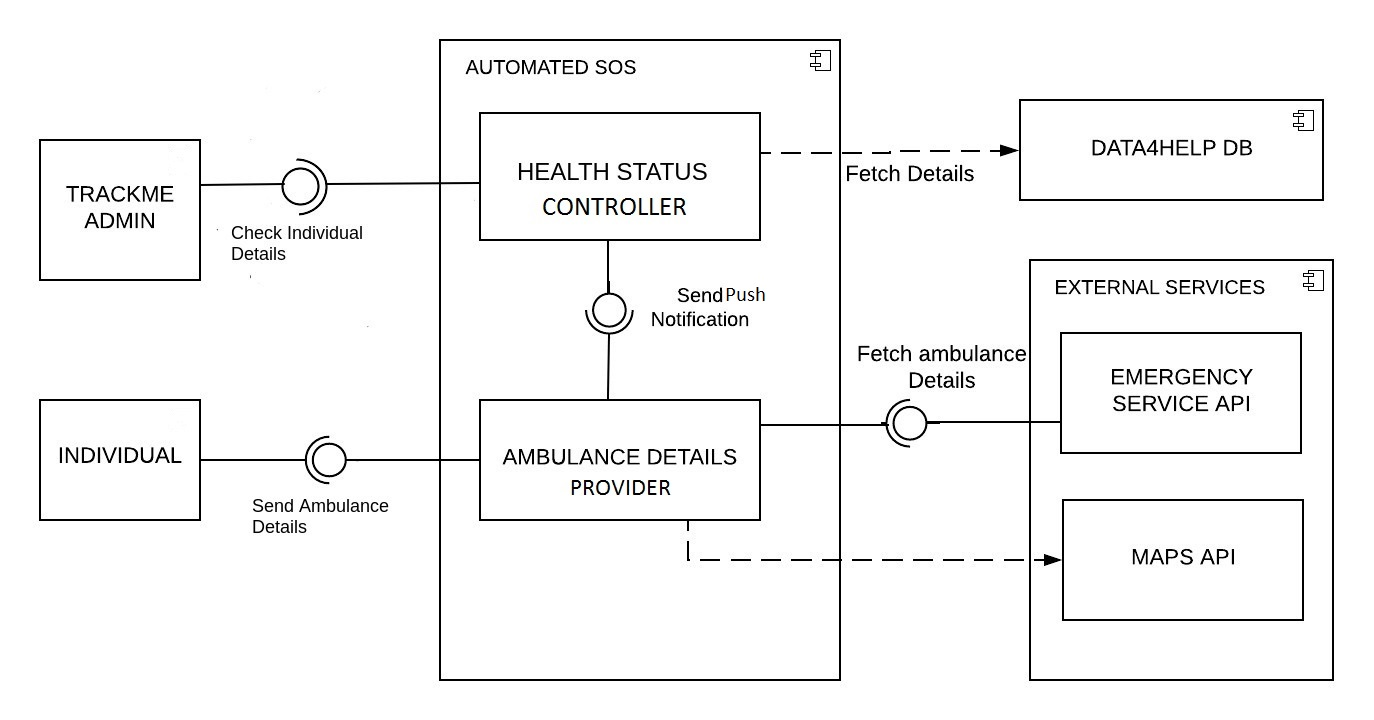
\includegraphics[width=\textwidth]{./DD_Diagrams/ComponentAutomatedSOS.jpg}
      	\caption{Component Diagram for AutomatedSOS Service}
        \label{TrackMe_c2}
	\end{center}
\end{figure}

\begin{itemize}
\item\textbf{Health Status Controller:}  uses the help of the Data4Help DB to get the details of an Individual. The TrackMe Admin provides an interface check Individual Details to the controller. The controller then, monitors the individual's vitals and when the vital is below the threshold value, it provides an interface named send notification.  
\item\textbf{Ambulance Details Provider:} gets the details of all the Ambulance associated to the major hospitals from the Emergency Service API. It uses the maps API to get the nearby ambulances and send notification to that ambulance driver application. It uses the functionality of Push Notification to send the notification. After a driver accept the request, the details of the driver is send to the Individual. 
\newline
\end{itemize}
\textbf{TRACK4RUN SERVICE}

\begin{figure}[H]
	\begin{center}
		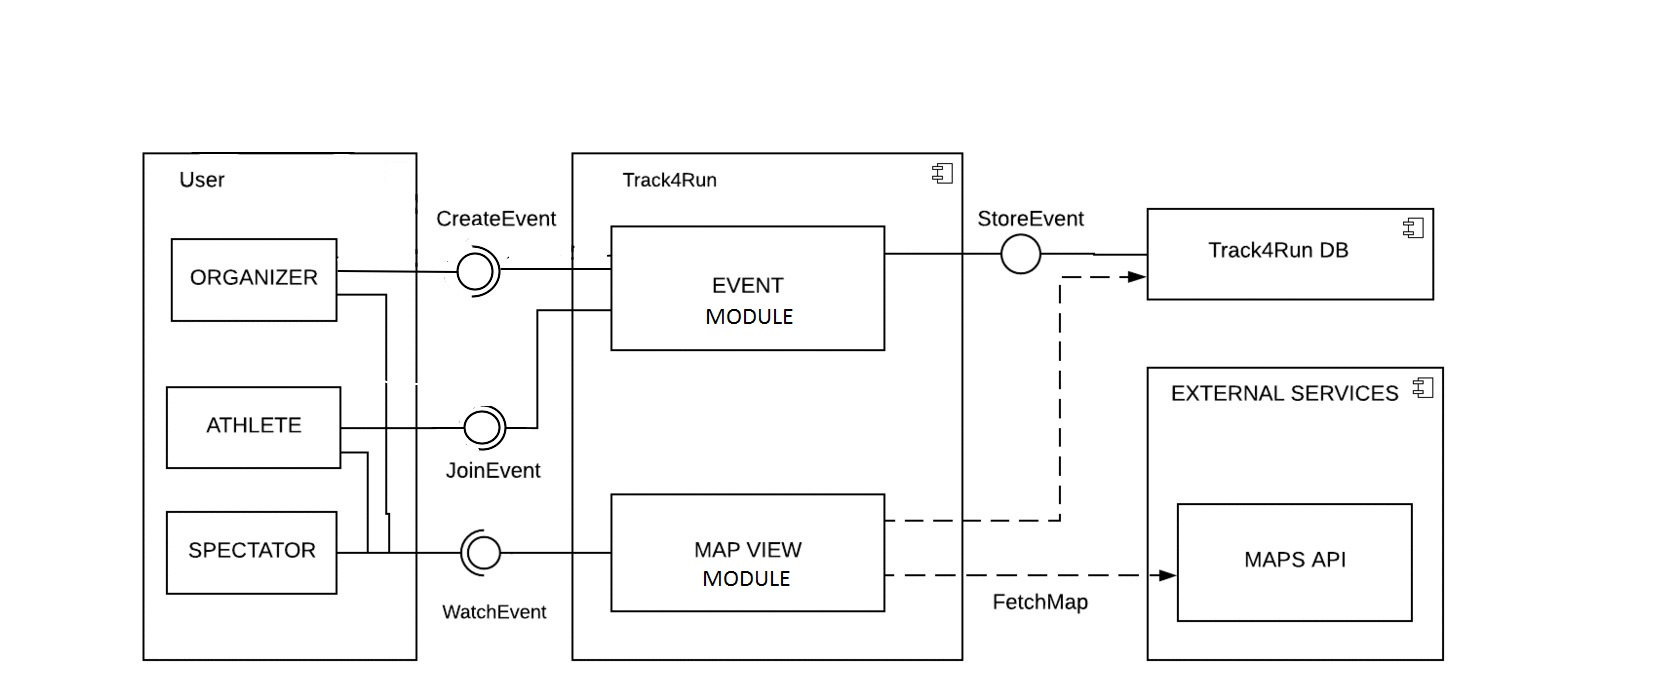
\includegraphics[width=\textwidth]{./DD_Diagrams/ComponentTrack4Run.jpg}
      	\caption{Component Diagram for Track4Run Service}
        \label{TrackMe_c3}
	\end{center}
\end{figure}

\begin{itemize}
\item\textbf{Event Module:} manages the details of the event and the athletes. It gets all the details of the event from the organizer which is entered after the organizer upgrades to the service. The event details is stored in the Track4Run DB. The athlete joins the event and is then associated with that specific event. 
\item\textbf{Map View Module:} It uses the Map API to provide an interface watch event to the organizer, athlete and the spectator. It checks the validity of the subscribed users. It uses the Track4Run DB to get the location of the athletes participating in an event, and then maps it to the interface.
\newline\newline\newline\newline\newline
\end{itemize}
\textbf{MAIN COMPONENT}

\begin{figure}[H]
	\begin{center}
		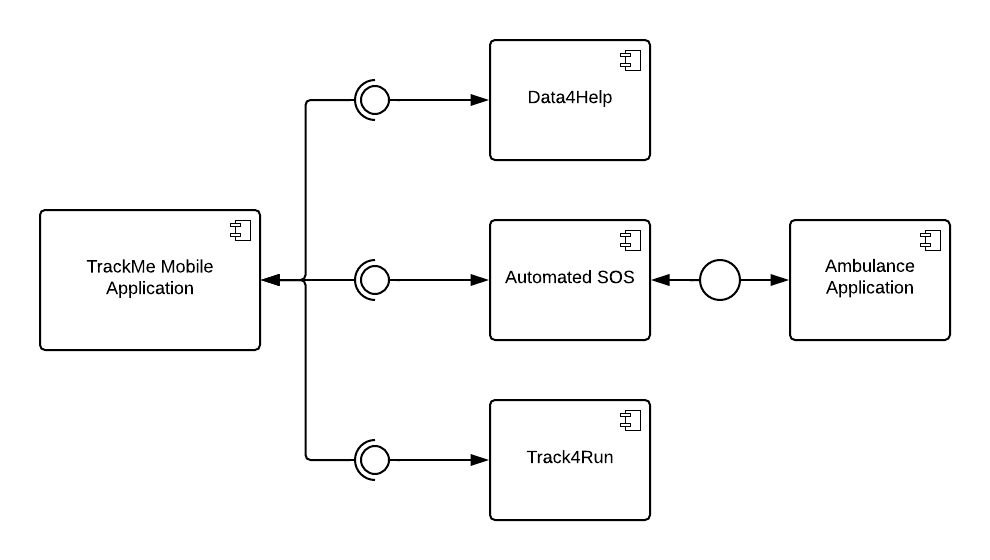
\includegraphics[width=\textwidth]{./DD_Diagrams/Component.png}
      \caption{Main Component Diagram}
        \label{TrackMe_c0}
	\end{center}
\end{figure}
The main component is divided into three subcomponents which are shown separately to avoid unreadability. All the three subcomponents are the services which is being provided by the TrackMe Application.\newline
The Ambulance Application is a separate application developed explicitly for the ambulance drivers where they receive individuals details through push notification. It is connected to Automated SOS service for exchange of information of ambulance and individual respectively.

\section{Deployment View}
\begin{figure}[H]
	\begin{center}
		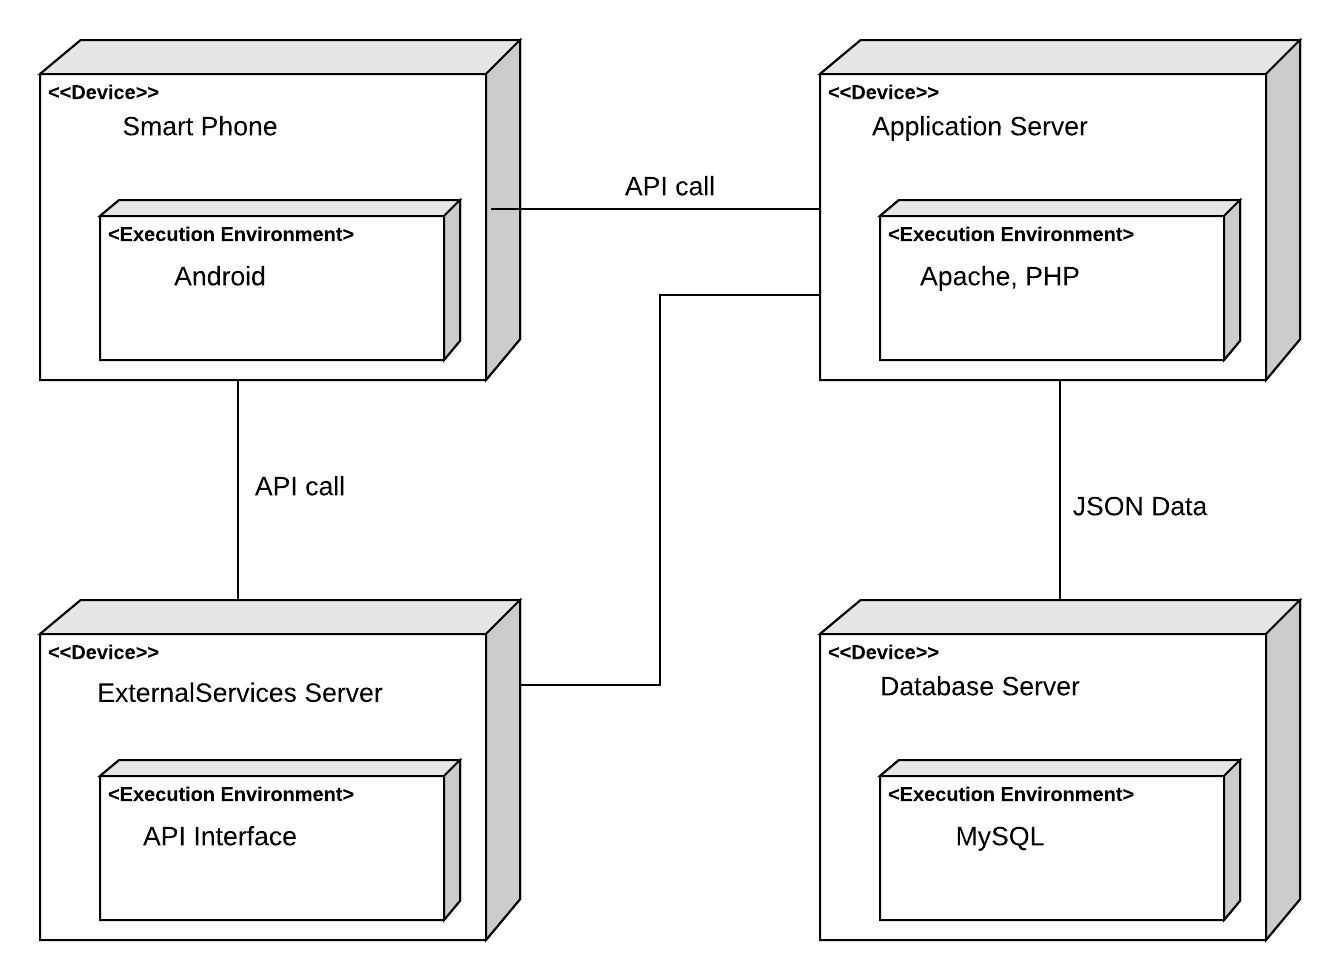
\includegraphics[width=\textwidth]{./DD_Diagrams/Deployment.png}
      \caption{Deployment Diagram}
        \label{TrackMe_depdia}
	\end{center}
\end{figure}
It shows architecture of the system as deployment (distribution) of software artifacts to deployment targets. Artifacts represent concrete elements in the physical world that are the result of a development process which are \textit{Android, Apache, PHP, API Interface} and \textit{MySQL}. Deployment target is usually represented by a node which is either hardware device or some software execution environment which are \textit{Smart Phone, Application Server, External Service Server} and \textit{Database Server}. The nodes are connected through communication paths to create networked systems of arbitrary complexity.\newline
The nodes an their respective artifacts are explained below:
\begin{itemize}
\item \textbf{Smart Phone:} The user uses smart phone to view the mobile application of the system. This is implemented in the execution environment Android which is artifact of this device.\newline
-\textit{Android:} The Android application can be built using any platform. It takes the information from external API's and the database server of the application to process and show information to the user using XML design techniques and Java Script codes.
\item \textbf{Application Server:} The Application Server is the host of the application and the database server. It is the central system of the entire application which manages the transfer and retrieval of data. The execution environment here is Apache and PHP.\newline
-\textit{Apache and PHP: } The Server does all the transaction on the database and manages the retrieval and transfer of data from and to database by using PHP code. We use PHP code to help convert the database into an API in JSON format which can be easily used by the application's front end to use the data.
\item \textbf{Database Server:} It stores all the data which is used by the application. The execution environment is MySQL.\newline
-\textit{MySQl:} MySQL database is used to store the details where the data can be easily stored from the form the user fills in the application. 
\item \textbf{ExternalServices Server:} It contains the information of all the external servers required by the application. The information from the server by using the API Interface.\newline
-\textit{API Interface:} The API provides the data in the JSON format which is fetched in the android platform by API call. 


\end{itemize}



\section{Runtime View}
The runtime view is explained with the help of sequence diagrams, which shows the interaction between the components during runtime in a time flow depicting the order of which function takes place after another. The function names are same as the interface in order to help to relate the component, their interaction and their behavior during runtime. The sequence diagram of the three major services of TrackMe are shown which comprises the entire functioning of TrackMe and integrates to make the complete application.\newline
Here are the three sequence diagrams which briefly summarizes the runtime of the application.
\begin{figure}[H]
	\begin{center}
		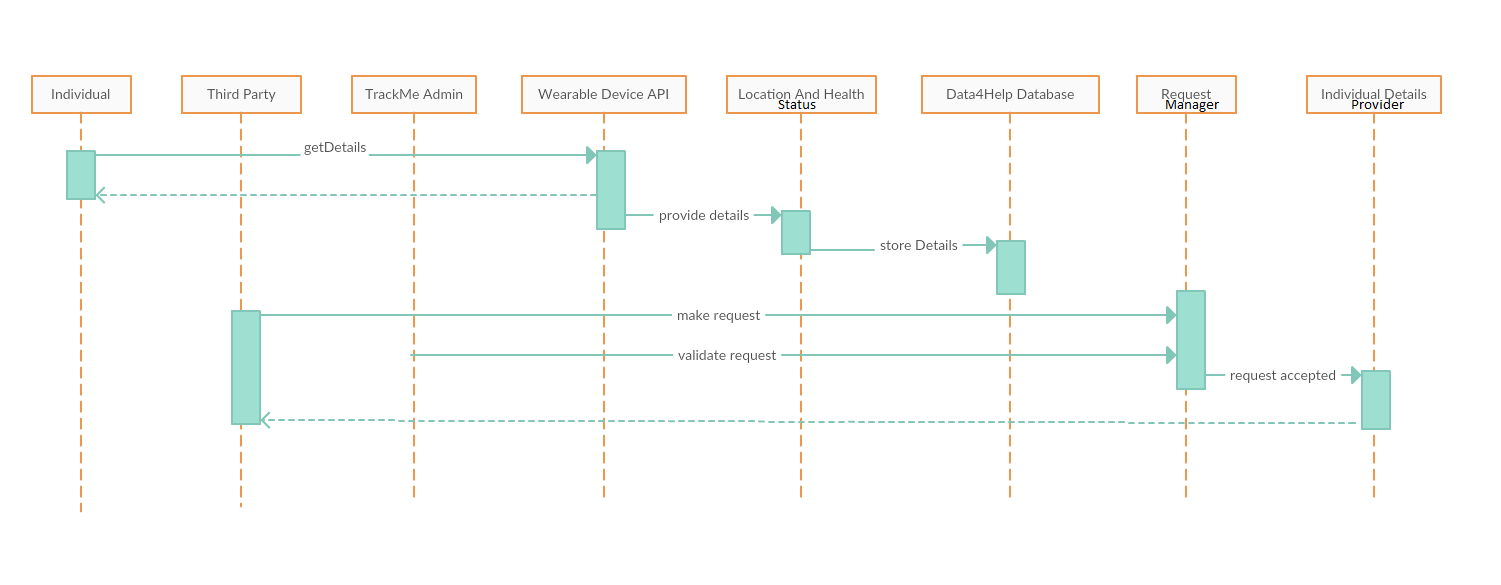
\includegraphics[width=\textwidth]{./DD_Diagrams/RuntimeData4Help.png}
      \caption{Sequence Diagram depicting runtime of Data4Help Service}
        \label{TrackMe_r1}
	\end{center}
\end{figure}
The location and health is taken from the user by the \textit{GetDetails Interface}  with the help of the API of the wearable device by \textit{ProvideDetails Interface}, which the individual selects from the list of compatible devices during registration. The details of the individual is then stored in the Data4Help database using \textit{StoreDetails Interface}.\newline
The thirdparty makes the request to access individual's data which is done by \textit{MakeRequest Interface}.\newline
The TrackMe Admin then validates the third party request and sends it to user to accept/reject or accepts/rejects himself according to the type of requests by \textit{ValidateRequest Interface}.\newline
If the request is accepted the user gets the access of the individual's details which uses the Data4Help Database in order to extract individual's details.
\begin{figure}[H]
	\begin{center}
		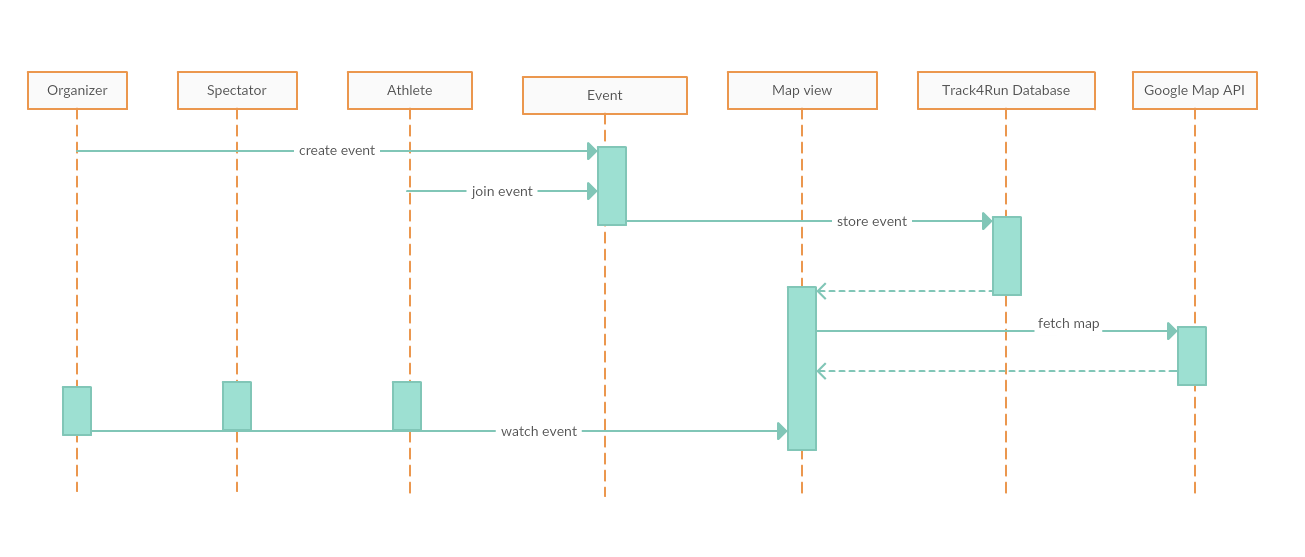
\includegraphics[width=\textwidth]{./DD_Diagrams/RuntimeAutomatedSOS.png}
      \caption{Sequence Diagram depicting runtime of AutomatedSOS Service}
        \label{TrackMe_r2}
	\end{center}
\end{figure}
Trackme checks the age of the user in order to know whether they are eligible for this service and checks the vitals to know about the emergency condition using  using \textit{CheckIndividualDetails Interface} which is fetched from the Data4Help Database and updated as Health Status component which contains the emergency vitals of individuals.\newline 
If the emergency situation is acknowledged the admin sends notification using \textit{SendPushNotification Interface} which includes the health status and location.\newline
The Individual receives the Ambulance Details by \textit{SendAmbulanceDetails Interface} and can track the ambulance whose information is fetched from the emergency Service API using \textit{FetchAmbulanceDetails Interface} and uses Maps API to show the map.
\begin{figure}[H]
	\begin{center}
		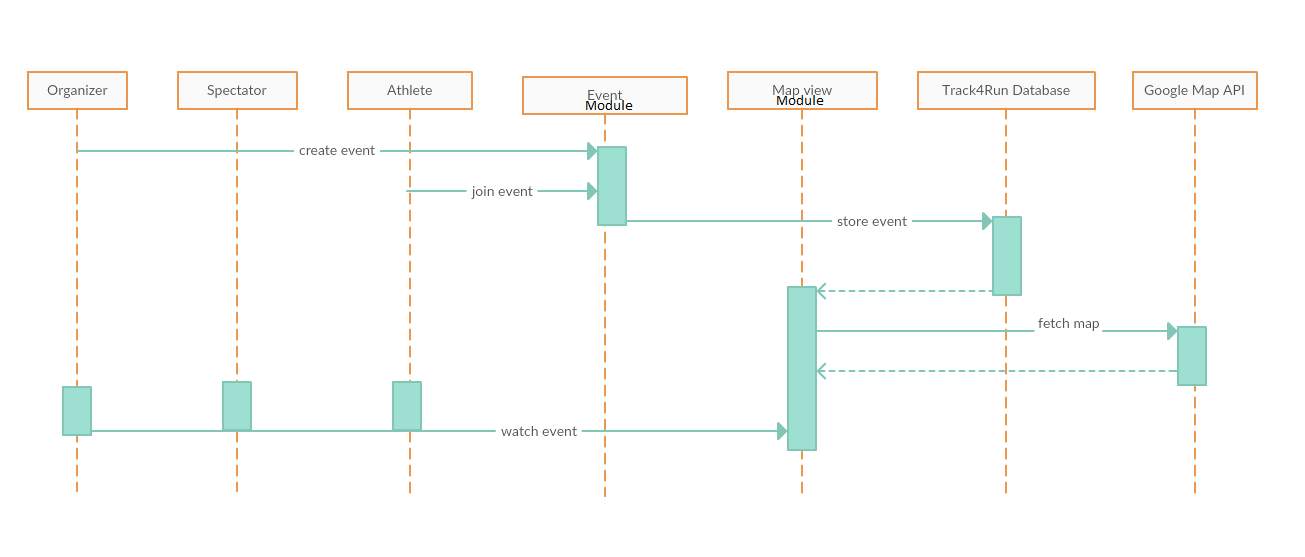
\includegraphics[width=\textwidth]{./DD_Diagrams/RuntimeTrack4Run.png}
      \caption{Sequence Diagram depicting runtime of Track4Run Service}
        \label{TrackMe_r3}
	\end{center}
\end{figure}
The organizer creates an event which the athlete joins using \textit{CreateEvent Interface} and \textit{JoinEvent Interface} respectively. The details of the event is store din the Track4Run Daatabase using \textit{StoreEvent Interface} which is used by Map view to show the details on map. The organizer, athlete and Spectator can watch the race in a map using \textit{WatchEvent Interface} which uses Map API to fetch the map.

\section{Component Interfaces}
In the following diagrams, the component interfaces are presented and the dependencies between the parts of the application server are shown. Each Interfaces which is already explained in the runtime view are detailed here with all the functions and methods they include. Like the component diagram, has three parts to implement three services in the same manner this has three separate diagram to explain all the interfaces and there interactions.
\begin{figure}[H]
	\begin{center}
		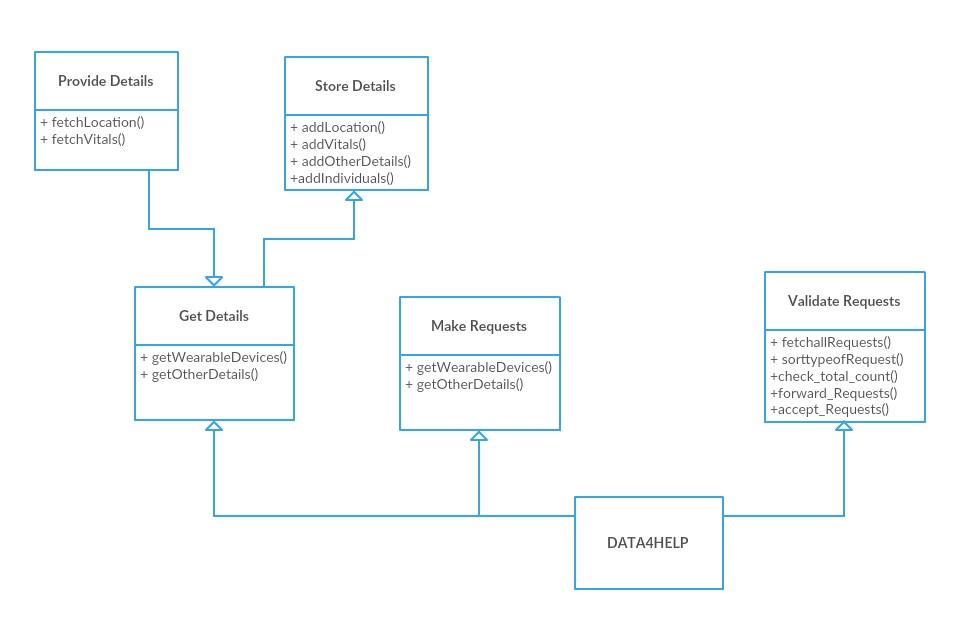
\includegraphics[width=\textwidth]{./DD_Diagrams/InterfaceData4Help.jpg}
      \caption{Component Interface Diagram for Data4Help}
        \label{TrackMe_int1}
	\end{center}
\end{figure}
\begin{figure}[H]
	\begin{center}
		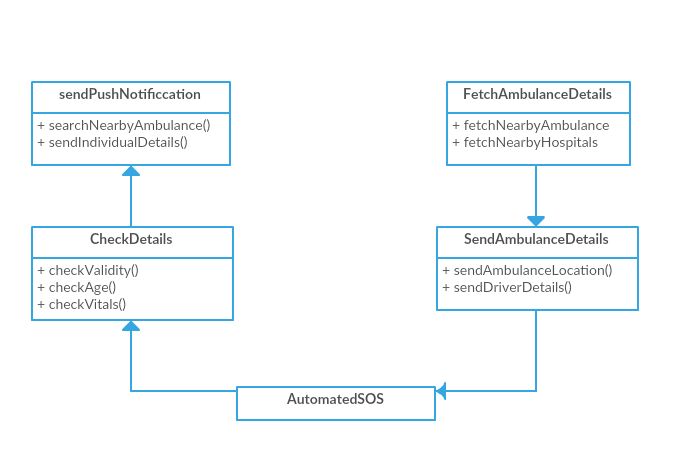
\includegraphics[width=\textwidth]{./DD_Diagrams/InterfaceAutomatedSOS.png}
      \caption{Component Interface Diagram for AutomatedSOS}
        \label{TrackMe_int2}
	\end{center}
\end{figure}
\begin{figure}[H]
	\begin{center}
		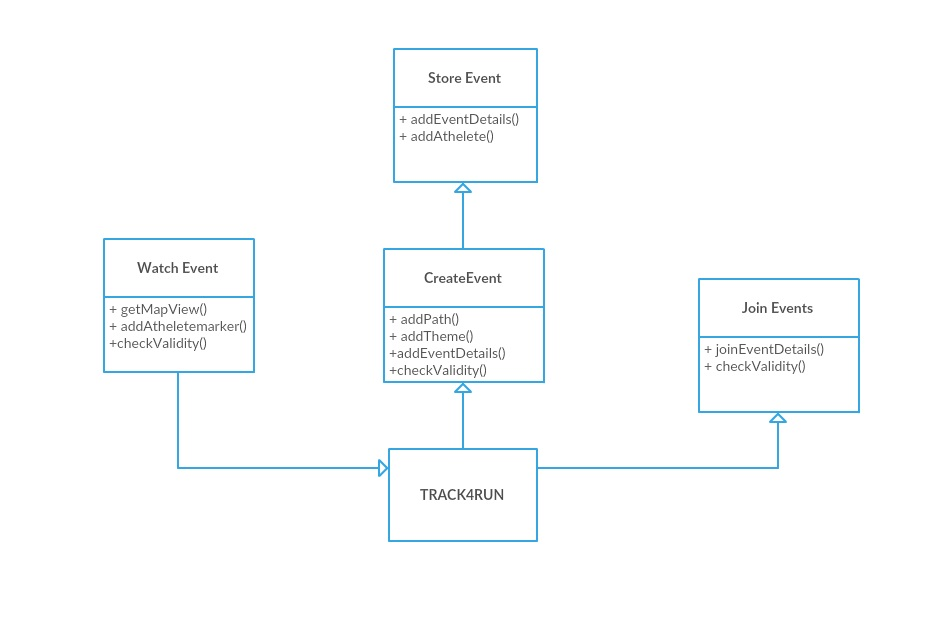
\includegraphics[width=\textwidth]{./DD_Diagrams/InterfaceTrack4Run.jpg}
      \caption{Component Interface Diagram for Track4Run}
        \label{TrackMe_int3}
	\end{center}
\end{figure}

\section{Selected architectural styles and patterns}
\subsection{Overview}

\qquad The system essentially uses a variety of the multi-layered architecture i,e is the three-tired architecture for our TrackMe application. The application includes a presentation layer, business layer and data layer. The presentation layer, which is the top most layer represents the  display of information related to the services given by the application like checking health status, requesting data, watching a live race etc. The presentation layer directly interacts with the client getting information from the client, with the help of GUI. The business layer also known as the application layer in general, fetches the details form the presentation layer and does detailed processing. For instance it ensures the connection with the corresponding external services required and processing for the data from the services like Google maps, wearable devices etc. The data access layers basically provides an API to the application tier that exposes methods of managing the stored data without exposing or creating dependencies on the data storage mechanisms.

\par We use a three tier application so that we would be able to update the technology stack of one tier without affecting the other one, and provides an easy of managing the different layers.

\subsection{Design Patterns and Architectural Choices}
\begin{enumerate}
\item Push Notification
\par We have used the push notifications, which include the location and details of the individuals in need of emergency care are send to the ambulance drivers via the ambulance application. We basically use the application to make sure of the time constraints that the notification should reach within 5 seconds. The choice is made because of the difficulty in coming up with an asynchronous protocol for message exchanging.
\item Robustness 
\par The principal usage of the system is done through mobile applications which are running on mobile terminals. As we can imagine, in that domain the robustness of the system is an important aspect to keep in
mind. The mobile devices are often subject to loss of connectivity and for that reason the communication between the server and a client could be not available in various time points
\end{enumerate}


\subsection{Other Design Decisions}
\begin{enumerate}
\item Storage of Passwords
\par The passwords are not stored in plain-text but they are hashed and salted with cryptographic hash functions. This provides a last line of defense in case of data theft.
\item Programming Languages
\par For the implementation of TrackMe application we choose Java as a programming language. This choice is based on the following considerations:
	\begin{enumerate}
	\item Java is a widespread programming language, so we are sure that there will be availability of skilled programmers in this technology.
    \item The choice of the platform is left to the developer. He/she has wide range of Java platforms to choose from.
	\end{enumerate}
\item Ambulance Mobile Application
\par The ambulance mobile application has been developed basically for the ambulance drivers to recieve the above mentioned push notification within a time interval of 5 seconds.
\item External Services
\par The system uses external services, Google Maps to offload all geo-localization, position tracking and map visualization process. The reasons of the choice are the following:
	\begin{enumerate}
	\item Manually developing maps for city of Milan is not a viable option due to tremendous amount of coding and data collection time required.
    \item Google Maps is a well-established, tested and reliable software component used by millions of people used around the world.
    \item Google Maps can be used both on the server side and the client side. 
    \item Users feel comfortable using a software which they daily use it.
    \item Google Maps offers API, enabling programmatic access to features.
	\end{enumerate}
    
\par The system also uses external services like wearable device API, which helps us to fetch the health vitals of the patients and the emergency service API to extract all the details of the nearby hospitals. Wearable device are the best choice to get the health vitals of a patient as it is easy to have it on hand always and can be easily connected to the application. Most of the users will be having a prior experience to use a wearable device.
\end{enumerate}



%%%%%% USER INTERFACE DESIGN %%%%%%%%
\chapter{User Interface Design}
\label{ch:user_interface_design}
The following User-Interface flow diagram enable us to model the high-level relationships between major user interface elements that are described in our RASD documents. It is used to organize the activities of TrackME application into groups and have an overview of the interfaces and interactions. \newline

\begin{itemize}
\item The user interface for an individual allows the individual to view the vitals, view the third party details, and accept/reject the request.
\begin{figure}[H]
	\begin{center}
		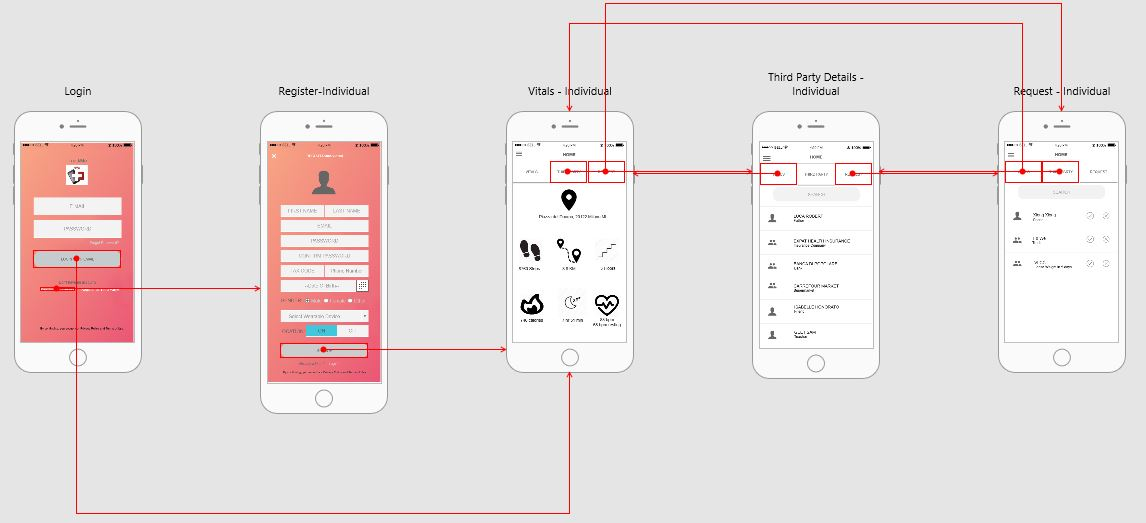
\includegraphics[width=\textwidth]{./DD_Diagrams/UI_Individual.JPG}
        \caption{User Interface - Individual}
        \label{ui_individual}
	\end{center}
\end{figure}
\end{itemize}

\begin{itemize}
\item The user interface for a Third Party allows the third party to view the details of the individual viewed in a pop-up box, allows to make new request, and view the status of the request already made.
\begin{figure}[H]
	\begin{center}
		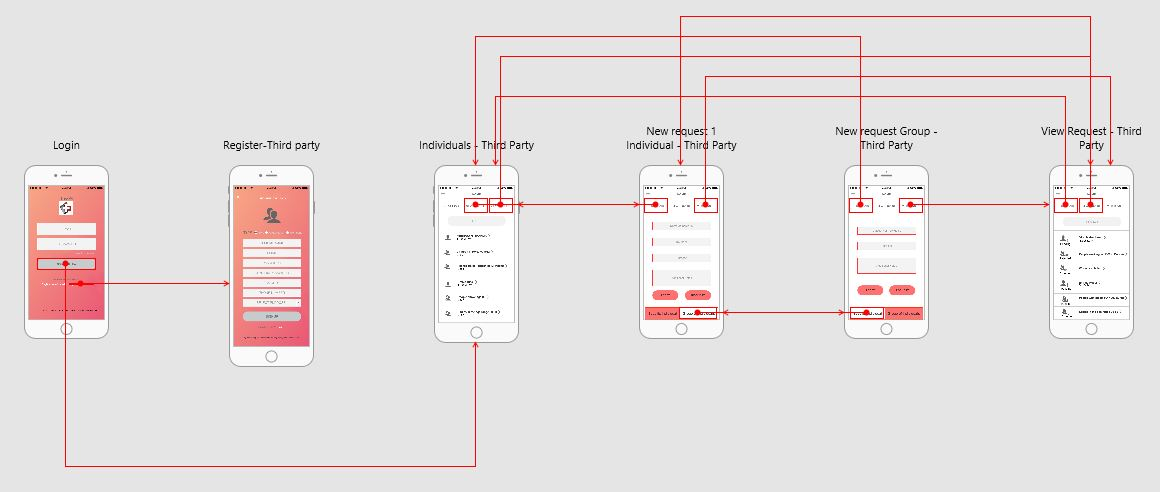
\includegraphics[width=\textwidth]{./DD_Diagrams/UI_ThirdParty.JPG}
        \label{ui_thirdparty}
        \caption{User Interface - Third Party}
	\end{center}
\end{figure}
\end{itemize}

\begin{itemize}
\item The Menu Interface allows an user to view their own profile, upgrade to a new service, and then allow to view the new service.
\begin{figure}[H]
	\begin{center}
		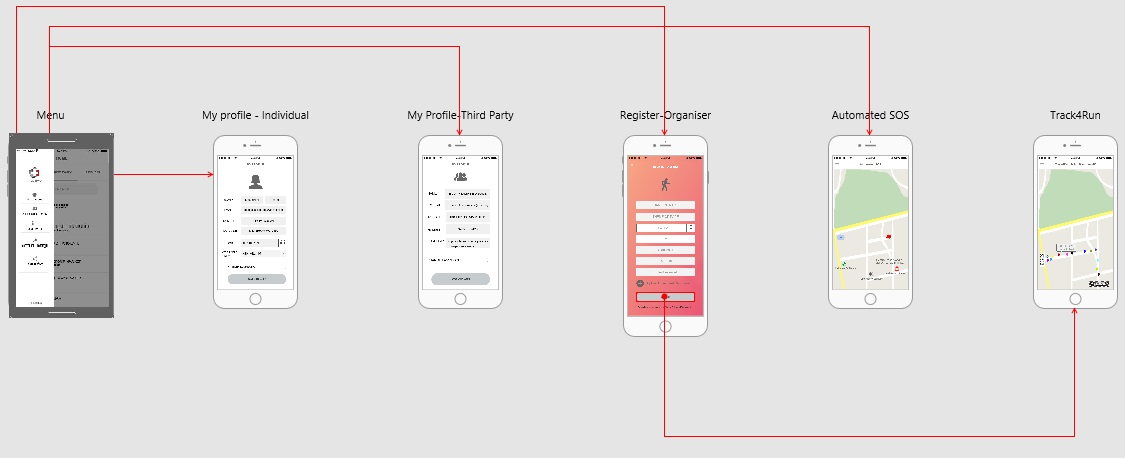
\includegraphics[width=\textwidth]{./DD_Diagrams/UI_Menu.JPG}
        \caption{User Interface - Menu}
        \label{ui_menu}
	\end{center}
\end{figure}
\end{itemize}




%%%%%% REQUIREMENTS AND TRACE ABILITY %%%%%%%%
\chapter{Requirements Traceability}
\label{ch:requirement_traceability}

The main objective of determining the design described in this document was to fulfill the requirements and goals mentioned in the Requirement Analysis and Specific Documents.\newline
The following list outline the mapping between the requirement and goals with the design elements mentioned in the DD.\newline

\begin{itemize}

\item\textbf{[G1]} Providing a list of the wearable devices that an individual can choose from. ([R1]-[R2])
\begin{itemize}
\item Data4Help
\begin{itemize}
\item Location Module
\item Health Module
\item Wearable Device API
\item Data4Help DB
\end{itemize}
\end{itemize}

\item\textbf{[G2]} Expedite the request made by the 3rd party to an individual to access their details. ([R3]-[R4])
\begin{itemize}
\item Data4Help
\begin{itemize}
\item Request Manager
\item Data4Help DB
\end{itemize}
\end{itemize}

\item\textbf{[G4]} Validating the request made by the 3rd party to provide the details of a group of individuals.([R6]-[R8])
\begin{itemize}
\item Data4Help
\begin{itemize}
\item Request Manager
\item Individual Details Provider
\item Data4Help DB
\end{itemize}
\end{itemize}

\item\textbf{[G5]} Quick access of the data to the 3rd party once the request is approved.([R9]-[R10])
\begin{itemize}
\item Data4Help
\begin{itemize}
\item Request Manager
\item Individual Details Provider
\item Data4Help DB
\end{itemize}
\end{itemize}

\item\textbf{[G6]} Immediate update of the data once an individual updates their own details.([R11]-[R12])
\begin{itemize}
\item Data4Help
\begin{itemize}
\item Location Module
\item Health Module
\item Wearable Device API
\item Data4Help DB
\end{itemize}
\end{itemize}

\item\textbf{[G8]} Monitoring the health status of the subscribed individual to the Automated SOS service.([R14]-[R16])
\begin{itemize}
\item AutomatedSOS
\begin{itemize}
\item Health Status Controller
\item Ambulance Details Provider
\item Data4Help DB
\item Emergency Service API
\item Maps API
\end{itemize}
\end{itemize}

\item\textbf{[G9]]}  Develops an interface to organize a race for the subscribed 3rd party to the Track4Run service.([R17]-[R19])
\begin{itemize}
\item Track4Run
\begin{itemize}
\item Event Module
\item Track4Run DB
\end{itemize}
\end{itemize}

\item\textbf{[G10]} Give access to the details of the race once an individual participate in it.([R20]-[R21])
\begin{itemize}
\item Track4Run
\begin{itemize}
\item Event Module
\item Track4Run DB
\end{itemize}
\end{itemize}

\item\textbf{[G11]} Live visualization of the race .([R22]-[R23])
\begin{itemize}
\item Track4Run
\begin{itemize}
\item MapView Module
\item Track4Run DB
\item Maps API
\end{itemize}
\end{itemize}

\end{itemize}

%%%%%% Implementation Integration and TestPlan %%%%%%%%
\chapter{Implementation, Integration and Test Plan}
\label{ch:implementaion_intergrationandtestplan}

\section{Implementation}
The implementation of the TrackMe system will be done service by service followed with the integration of all the services. The order in which it is be carried out depends on a number of factors like the complexity of the modules and services, the dependence of other modules on the component being implemented and to the system as a whole, and it should also take into account the possibility of discovering flaws with the proposed design. The later should be dealt in a way that, if such an unfortunate event does happen,the flaws should be found and corrected as soon as possible, to limit the cost of the change of design. 
In this sense, the components of the TrackMe, could be grouped in the following way, with the order specifying the order of implementation: \newline
1. Data4Help Service\newline 2. Automated SOS Service and Ambulance Application\newline 3. Track4Run Service\newline 4. TrackMe (Connecting the above three services)\newline

The first service to be built is Data4Help Service as the further services exploits the features of Data4Help Service. Data4Help is a base service which all the individuals and third party will have by default when they register in the application. Hence, it has to be built first as a separate service. This service does the main function of taking data from user and storing it in database and hence does not require any payment interface with might be required by other services, hence it is implemented separately.\newline 

After the first service AutomatedSOS and TrackMe Ambulance Application is implemented which is a service used by only Individuals. This is a service for the elderly individuals whose vitals are monitored and a nearby ambulance is sent whenever emergency situations are encountered. This service exploits the features of the above service and hence it is implemented after that. The details of the individuals with vitals below threshold is sent to the Ambulance Driver. The ambulance drivers have explicit applications in order to ensure fast delivery of individual's data through push notification.Hence the application must be implemented together with this service layer as there is an exchange of information from application to this service layer and vice versa.\newline

The next service implemented is Track4Run service which is basically an event which is organized by Organizers who are basically third party and individuals can perform as athlete. This service is not related to the second service by any means and hence both the services can be implemented parallely and separately and this can be implemented even before AutomatedSOS. The order of these two service wont matter but it must be implemented after Data4Help Service as it exploits the feature of that service as well.\newline

After implementing all the three services of the application, we can merge them and implement the entire working of the application connecting all the three services and how the user upgrades from Data4Help to other services and uses them. Hence this layer is implemented at the end after implementing all the services separately.

\section{Integration}
\textbf{1. Integration of Data4Help} 
\begin{itemize}
\item Integration of the components of Data4Help of the application server.\newline
-- Request Manager, Individual Details Provider
\item Integration of components of Data4Help with the DBMS. \newline
-- Location Module, Data4Help DB\newline
-- Health Module, Data4Help DB\newline
-- Individuals Details Provider, Data4Help DB
\item Integration of components of Data4Help with the (other) external services. \newline
-- Location Module, Wearable Device API\newline
-- Health Module, Wearable Device API\newline
\end{itemize}
\textbf{2. Integration of Automated SOS}
\begin{itemize}
\item Integration of the components of Automated SOS of the application server.\newline
-- Health Status Controller, Ambulance Details Provider
\item Integration of components of Automated SOS with the DBMS. \newline 
-- Health Status Controller, Data4Help DB
\item Integration of components of Automated SOS with the (other) external services. \newline
-- Ambulance Details Provider, Emergency Services API\newline
-- Ambulance Details Provider, Maps API\newline
\end{itemize}
\textbf{3. Integration of Track4Run}
\begin{itemize}
\item Integration of components of Track4Run with the DBMS. \newline 
-- Event Module, Track4Run DB
\item Integration of components of Track4Run with the (other) external services. \newline
-- Map View Module, Track4Run DB
-- Map View Module, Maps API
\end{itemize}
\textbf{4. Integration of TrackMe}
\begin{itemize}
\item Integration of the components of TrackMe with Data4Help.
\item Integration of components of TrackMe with AutomatedSOS. 
\item Integration of components of TrackMe with Track4Run. 
\item Integration of AutomatedSOS with TrackMe Ambulance Application.
\end{itemize}

\section{Integration Test Plan}
\begin{figure}[H]
	\begin{center}
		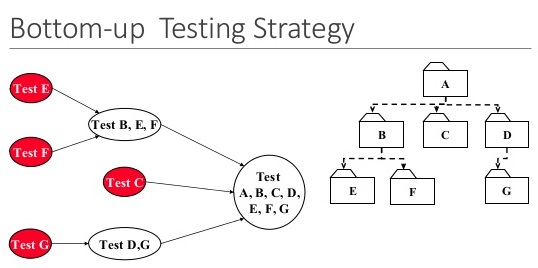
\includegraphics[width=\textwidth]{./DD_Diagrams/testplan2.jpg}
      \caption{Bottom up- strategy for testing integration plan}
        \label{TrackMe_tp2}
	\end{center}
\end{figure}
A bottom-up approach is the piecing together of systems to give rise to more complex systems, thus making the original systems sub-systems of the emergent system. Bottom-up processing is a type of information processing based on incoming data from the environment to form a perception. From a cognitive psychology perspective, information enters the eyes in one direction (sensory input, or the "bottom"), and is then turned into an image by the brain that can be interpreted and recognized as a perception (output that is "built up" from processing to final cognition). In a bottom-up approach the individual base elements of the system are first specified in great detail. These elements are then linked together to form larger subsystems, which then in turn are linked, sometimes in many levels, until a complete top-level system is formed. This strategy often resembles a "seed" model, by which the beginnings are small but eventually grow in complexity and completeness. However, "organic strategies" may result in a tangle of elements and subsystems, developed in isolation and subject to local optimization as opposed to meeting a global purpose.\newline
Considering the implementation plan and the overall architecture of the TrackMe application, the chosen strategy for the integration testing is the \textit{bottom-up strategy}. This allows us to start the integration and it’s testing while not waiting for the completion of the development and the unit testing of each component in the system. Considering the integration of two components, we would assume that, in best case, they have been implemented fully and that their respectful unit tests pass. However, the integration can, in some cases, start, if necessary, before the implementation has been completed. This can be allowed if the part of the component needed for that specific integration has been completed and tested. \newline

Since the opted solution is to start from the bottom-up, that means that the among the first integrations performed will have the already built external components in them. Since the application rests on these services and the communication with them, this order of integration and testing will enable the earlier detection of errors in these critical parts. 
\begin{figure}[H]
	\begin{center}
		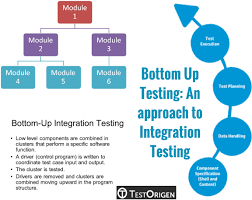
\includegraphics[width=\textwidth]{./DD_Diagrams/testplan.png}
      \caption{Working of bottom up- strategy for testing integration plan}
        \label{TrackMe_tp}
	\end{center}
\end{figure}

%%%%%% EFFORT SPENT%%%%%%%%
\chapter{Effort}
\label{ch:effort}

\section{Hours of Work}
\subsection{Saloni Kyal}
\begin{table}[H]
	\centering
    \begin{tabular}{|l|l|l|}
    \hline
     \textbf{Date} & \textbf{Task} & \textbf{Hours}\\
    \hline
    22-11-18 & Analyze DD Document and Decide Architecture (Group Work) & 3 \\
    \hline
	01-12-18 &  Component Diagram and Runtime View(Group work) &  8\\
    \hline
    02-12-18 &  Deployment and DD Documentation  &  3\\
    \hline
    05-12-18 &  Implementation plan, integration and testing  &  4\\
    \hline
		06-12-18 & Component Diagram documentation(Group work) & 3\\
        \hline
        07-12-18 & Requirement Traceability and Automated Component interface & 1\\
        \hline
		08-12-18 & Documentation and RASD version 2(Group work) & 8\\
    \hline
	& \textbf{Total}	& \textbf{30}\\   
    \hline
    \end{tabular}
\end{table}

\subsection{Mohini Gupta}
\begin{table}[H]
	\centering
    \begin{tabular}{|l|l|l|}
    \hline
     \textbf{Date} & \textbf{Task} & \textbf{Hours}\\
    \hline
    22-11-18 & Analyze DD Document and Decide Architecture (Group Work) & 3 \\
    \hline
	01-12-18 &  Component Diagram and Runtime View(Group work) &  8\\
    \hline
    03-12-18 &  User Interface Design &  4\\
     \hline
        05-12-18 & Requirement Traceability & 1\\
    \hline
		06-12-18 & Component Diagram documentation(Group work) & 3\\
        \hline
		06-12-18 & Documentation & 3\\
        \hline
		08-12-18 & Documentation and RASD version 2(Group work) & 8 \\
    \hline
	& \textbf{Total}	& \textbf{30}\\   
    \hline
    \end{tabular}
\end{table}

\subsection{Haritha Harikumar}
\begin{table}[H]
	\centering
    \begin{tabular}{|l|l|l|}
    \hline
     \textbf{Date} & \textbf{Task} & \textbf{Hours}\\
    \hline
    22-11-18 & Analyze DD Document and Decide Architecture (Group Work) & 3 \\
    \hline
    25-11-18 & Introduction, Scope and Details & 1\\
    \hline
	01-12-18 &  Component Diagram and Runtime View(Group work) &  8\\
    \hline
    03-12-18 & Software Component Diagram Final & 1\\
    \hline
		06-12-18 & Component Diagram documentation(Group work) & 3\\
        \hline
        07-12-18 & Component Interface Diagram & 2\\
        \hline
		08-12-18 & Documentation and RASD version 2(Group work) & 8\\
        \hline
        08-12-18 & System Architecture and other design constraints & 2\\
        \hline
        09-12-18 & Final Draft & 2\\
    \hline
	& \textbf{Total}	& \textbf{30}\\   
    \hline
    \end{tabular}
\end{table}

\chapter{References}
\begin{itemize}
\item Specification Document: "Mandatory Project Assignment AY 2018-2019"
\item Lucid Chart Tutorials 
\item Design Slides
\end{itemize}


%\appendix
%\chapter{Appendix}`'
%\input{appendix.tex}

%\input{bibilography.tex}

\end{document}